\chapter{Metodologia}  \label{cap:03}

Este trabalho caracteriza-se como uma pesquisa aplicada de natureza experimental. Define-se como aplicada pois aborda um problema prático concreto - a carência de aplicativos capazes de descrever ambientes para pessoas com deficiência visual em tempo real — e busca, simultaneamente, promover a inclusão desse grupo minoritário no uso de IA. Já seu caráter experimental advém do desenvolvimento de um protótipo e da comparação de diferentes modelos de IA para a tarefa de descrição de imagens.

No que se refere à abordagem metodológica, há uma componente quantitativa, evidenciada na coleta de métricas (por exemplo, medição de latência e análise das descrições por meio de indicadores específicos) e na comparação estatística dos resultados entre os modelos. Em paralelo, há aspectos qualitativos na avaliação da coerência das legendas geradas, embora, nesta etapa, os testes tenham sido realizados apenas internamente pelo autor.

\section{Ferramentas e Tecnologias}

Nesta seção, descrevem-se os recursos de \textit{hardware}, \textit{software} e bibliotecas utilizados no desenvolvimento do aplicativo e na execução dos modelos de IA.

\subsection{\textit{Hardware} utilizado}

Para hospedar a API (Application Programming Interface) e oferecer suporte ao processamento dos modelos de LLM, utilizou-se um \textit{desktop} instalado no Instituto Federal de Mato Grosso do Sul (IFMS), Campus Três Lagoas. Esse computador apresenta as seguintes configurações:

\begin{itemize}
    \item \textbf{CPU:} 11th Gen Intel(R) Core(TM) i7-11700KF (8 núcleos físicos, 16 \textit{threads}, até 5,0 GHz)
    \item \textbf{GPU:} NVIDIA GeForce RTX 3070 (8 GiB de memória VRAM), Driver 550.107.02, suporte a CUDA 12.4
    \item \textbf{Memória:} 32 GiB DDR4
    \item \textbf{Armazenamento:} 1 TiB em SSD NVMe + RAID 5 (2,27 TiB) para armazenamento de dados
    \item \textbf{Sistema Operacional:} Debian GNU/Linux 12 (Bookworm), Kernel 6.1.0-13-amd64
\end{itemize}

Embora seja um ambiente favorável a testes com modelos de IA, a memória de 8 GiB da GPU pode se tornar um fator limitante para modelos de linguagem maiores. Além disso, a execução via CPU, caso o modelo exceda a capacidade da GPU, tende a prejudicar a latência das requisições. Nesse sentido, reforça-se o caráter experimental do desenvolvimento, pois a viabilidade plena da solução em cenários mais complexos depende de recursos computacionais adicionais, além de técnicas de otimização de modelos, como a quantização, que serão utilizadas para melhorar a performance neste projeto.

A quantização se apresenta como uma solução essencial para reduzir o consumo de memória e melhorar a eficiência computacional de redes neurais, tornando possível a execução de modelos de grande porte em dispositivos com recursos limitados. De acordo com \citeonline{Wei2024}, essa técnica permite diminuir a largura de banda necessária para a transmissão de dados e otimiza a velocidade de inferência sem comprometer significativamente a precisão dos modelos.

De forma geral, seguindo a definição de \citeonline{Wei2024}, a quantização é o processo de conversão de redes neurais que utilizam números de ponto flutuante em redes neurais de largura de bits reduzida, geralmente inteiras, com o objetivo de minimizar o custo computacional e o consumo de energia, tornando viável a implantação de modelos em ambientes de computação de borda. Assim, ao adotar essa técnica, busca-se equilibrar desempenho e eficiência, permitindo a execução otimizada do modelo no \textit{hardware} disponível.

\subsection{Aplicativo \textit{mobile}}

Para o módulo de aplicativo, foram consideradas ferramentas que aliassem eficiência no desenvolvimento e aderência aos requisitos do projeto, sobretudo o de desenvolver uma solução multiplataforma (Android e iOS). A partir dessas premissas, optou-se pelo \textit{framework} Flutter, conhecido, principalmente, por sua produtividade, trazendo agilidade na construção do aplicativo tanto para iOS como para Android, e uma comunidade ativa, onde é disponibilizado um amplo conjunto de pacotes e bibliotecas que aceleram o desenvolvimento.

Dentre as bibliotecas utilizadas, destacam-se:

\begin{itemize}
    \item \textbf{\texttt{flutter\_tts}:} Responsável pela conversão de texto em fala (TTS).
    \item \textbf{\texttt{flutter\_sound}:} Permite a gravação de áudios, viabilizando a utilização do áudio para o usuário questionar o que está na sua frente.
    \item \textbf{\texttt{camera}:} Facilita o acesso à câmera do dispositivo, para captura de imagens.
    \item \textbf{\texttt{http}:} Simplifica a realização de requisições REST à API desenvolvida em Python.
\end{itemize}

A escolha do Flutter visa garantir acessibilidade e praticidade no desenvolvimento, além de oferecer pacotes para a conexão direta com o \textit{hardware}, algo que é essencial para o projeto e garantia da usabilidade pelo usuário nos diferentes sistemas operacionais móveis.

\subsection{API}

O módulo da API foi implementado com o intuito de receber as imagens e os áudios do aplicativo, processá-los por meio de modelos de IA e retornar as descrições geradas, para, posteriormente, serem reproduzidos pelo aplicativo novamente. Para isso, adotou-se a linguagem Python, na versão 3.11.2, devido à ampla disponibilidade de bibliotecas de \textit{Machine Learning} e à gama de suporte existente da comunidade. Além do exposto, aliado à grande comunidade de desenvolvedores em Python, soma-se a disponibilidade de \textit{frameworks}, que visa trazer eficiência para o desenvolvimento. Desta forma, para este trabalho foi utilizado o \textit{framework web} FastAPI, que simplifica a criação de \textit{endpoints} REST (Representational State Transfer API) e facilita a escalabilidade e manutenção do servidor.

No servidor, os modelos ficam salvos, e o aplicativo se comunica com eles por meio da API hospedada no próprio servidor. A API fica responsável por:

\begin{enumerate}
    \item Receber a imagem e o áudio vindos do aplicativo Flutter, via requisição HTTP.
    \item Transcrição do áudio recebido com o questionamento sobre o ambiente.
    \item Pré-processar a imagem (por exemplo, redimensionar, normalizar).
    \item Executar o modelo de LLM escolhido para gerar a descrição da imagem.
    \item Retornar o texto descritivo ao aplicativo, que então o converte em áudio por meio do \texttt{flutter\_tts}.
\end{enumerate}

A flexibilidade do Python e do FastAPI permite alternar rapidamente entre diferentes modelos de IA, facilitando o processo de \textit{benchmark} e garantindo a modularidade do sistema.

\subsection{Modelos de IA}

Para a tarefa de descrição de imagens, este trabalho faz uso de três LLMs de código aberto disponíveis no Hugging Face:

\begin{itemize}
    \item \textbf{\texttt{Qwen/Qwen2.5-VL-7B-Instruct}:} possui um tamanho de 7 bilhões de parâmetros. Isto balança bom desempenho em legendagem de imagens com latência moderada, podendo ser executado em GPU de 8 GiB.
    \item \textbf{\texttt{llava-hf/llava-v1.6-mistral-7b-hf}:} também com 7 bilhões de parâmetros. Tem se destacado em instruções multimodais e apresenta boa relação entre desempenho e consumo de recursos, além de sua arquitetura ser utilizada por diversos outros modelos.
    \item \textbf{\texttt{meta-llama/Llama-3.2-11B-Vision-Instruct}:} possui 11 bilhões de parâmetros. Capaz de descrever melhor as imagens, porém mais exigente em termos de memória e processamento, podendo afetar a latência e o consumo de GPU.
\end{itemize}

Já para o processamento do áudio, ou seja, o processo de STT, também foi utilizado um modelo do Hugging Face, mais especificamente o modelo \texttt{openai/whisper-small} \cite{radford2023}. Este modelo foi escolhido por conta da sua grande capacidade de fazer transcrições, mesmo sendo um modelo pequeno, o que economiza recursos do \textit{desktop} disponível.

Cada modelo é carregado em Python por meio das bibliotecas Transformers (Hugging Face) e PyTorch, permitindo alternar rapidamente entre as opções durante os testes. A motivação para essa variedade de modelos é evidenciar as vantagens e limitações de cada abordagem em termos de acurácia descritiva e velocidade de processamento, reforçando o caráter experimental do desenvolvimento.

Os modelos foram escolhidos de forma empírica, visando principalmente garantir que seria possível a execução na máquina disponibilizada. Outros modelos também poderiam ser testados, porém, para efeitos de prototipagem, foram selecionados os três supracitados.

\subsection{TTS}

O processo do TTS é imprescindível para tornar as descrições de ambiente acessíveis a pessoas com deficiência visual utilizando IA. Neste projeto, optou-se por executar o TTS diretamente no aplicativo \textit{mobile}, visando, principalmente, a redução da latência e dos dados trafegados via rede, assegurando, desta forma, que o usuário possa receber a mensagem mesmo em conexões mais instáveis.

Para isso, empregou-se a biblioteca \texttt{flutter\_tts}, amplamente utilizada em aplicações Flutter. Ela foi escolhida tanto por sua integração simples em aplicativos como também pelas opções de customização, que podem facilmente ser ajustadas. 

Assim, o processo de descrição ocorre em duas etapas: (1) o servidor gera o texto com a descrição da imagem capturada e (2) o aplicativo recebe essa legenda e chama a função de TTS para sintetizar a fala em tempo real.

\section{Arquitetura do Sistema}

A fim de integrar de forma coerente o aplicativo \textit{mobile} e o servidor que hospeda os modelos de IA, projetou-se uma arquitetura orientada a serviços, conforme ilustrado na Figura \ref{fig:6}. Nela, o fluxo de dados segue as seguintes etapas: (1) captura de imagem e do áudio por meio de um gatilho, que foi definido como o toque na tela, (2) realização da requisição à API enviando a imagem e o áudio capturados, (3) o áudio é convertido em texto, por meio do modelo STT, (4) processamento pelo modelo LLM, (5) retorno do texto descritivo ao aplicativo e (6) conversão desse texto em fala (TTS).

\begin{figure}[!ht]
     \caption{Arquitetura do sistema (alto-nível)}
     \centering
     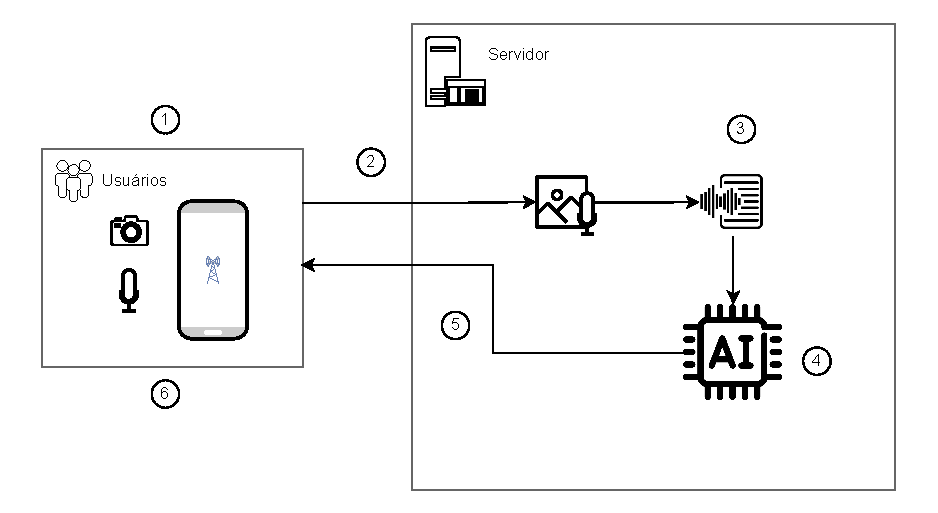
\includegraphics[width=0.7\linewidth]{imagens/architeture-tcc.drawio.pdf}
     \label{fig:6}
     \footnote{\textbf{Fonte:} Elaborado pelo Autor (2025)}
\end{figure}

Observa-se, portanto, que a arquitetura proposta facilita a interação entre Aplicativo (Flutter), API (FastAPI) e Modelos de IA para a descrição de imagens e o processamento de áudio. A abordagem orientada a serviços permite escalabilidade e manutenção simplificadas, já que cada componente (captura da imagem, conversão de áudio em texto, geração de legenda via LLM e TTS) pode ser atualizado ou substituído independentemente, sem impactar as demais partes do sistema.

\begin{figure}[!h]
     \caption{Diagrama de Sequência}
     \centering
     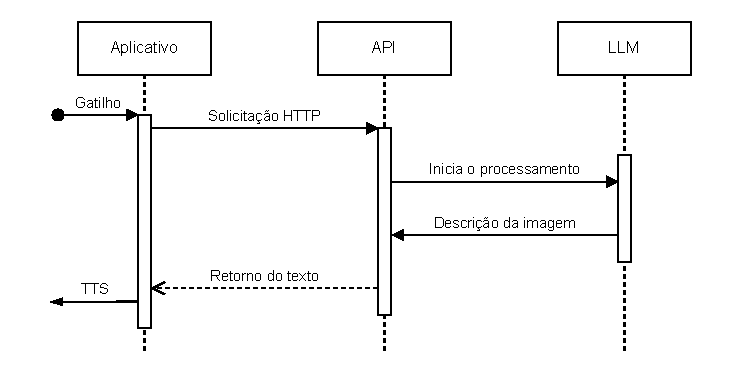
\includegraphics[width=0.7\linewidth]{imagens/diagrama_sequencia.drawio.pdf}
     \label{fig:7}
     \footnote{\textbf{Fonte:} Elaborado pelo Autor (2025)}
\end{figure}

A Figura \ref{fig:7} complementa a visão geral apresentada na Figura \ref{fig:6} ao detalhar, em formato de diagrama de sequência, as trocas de mensagens e o encadeamento temporal das chamadas entre o aplicativo, servidor e o LLM. Dessa forma, fica evidenciado que o processo se inicia na captura de multimídia (imagem e áudio), passa pelo envio dos dados à API e pela execução dos modelos de STT e LLM, e retorna ao aplicativo na forma de texto, convertido em áudio pelo TTS. Esse fluxo modular possibilita, ainda, testes de \textit{benchmark} para avaliar diferentes configurações ou modelos de IA sem a necessidade de alterações estruturais no aplicativo móvel.

\section{Procedimentos de Desenvolvimento}

Nesta seção, descreve-se o passo a passo para o desenvolvimento do protótipo, abrangendo desde a captura da imagem e a gravação de áudio no aplicativo Flutter até o retorno da descrição em áudio, com ênfase no processo de modularização que viabiliza a comparação de diferentes modelos de IA. O detalhamento segue a lógica de comunicação entre os módulos, já ilustrada na Figura \ref{fig:7}.

\subsection{Aplicativo}

Conforme destacado em seções anteriores, a escolha do \textit{framework} Flutter para o desenvolvimento do aplicativo se deve à necessidade de atender múltiplas plataformas (Android e iOS) de forma eficiente. Antes de iniciar a construção efetiva do aplicativo, procedeu-se a um planejamento detalhado para definir o melhor gatilho de captura, levando em conta que processos contínuos, disparados automaticamente, trariam um custo elevado tanto em termos de arquitetura quanto de processamento.

Inicialmente, cogitou-se o uso dos botões de volume como disparadores, mas concluiu-se que tal solução interferiria na alteração do volume do dispositivo, comprometendo a usabilidade. Por fim, optou-se pelo toque na tela, em que um primeiro toque inicia a gravação de áudio e a captura da imagem, e um segundo toque encerra a gravação, sinalizando que todo o material coletado (imagem e áudio) deve ser enviado à API.

Em termos de \textit{design} e construção de telas, decidiu-se que, dada a natureza do aplicativo — voltado para pessoas com deficiência visual —, uma interface minimalista seria mais adequada. Nesse sentido, retoma-se o argumento de \citeonline{Torres2002}, segundo o qual a usabilidade para esse público requer interfaces enxutas e objetivas. Assim, a aplicação conta basicamente com uma única tela, exibindo a câmera em tempo real. O usuário toca na tela para iniciar a coleta de dados (imagem e áudio) e, ao tocar novamente, finaliza o processo e envia todo o conteúdo ao servidor. As instruções de uso do aplicativo serão dadas por meio da biblioteca \texttt{flutter\_tts}, que permitirá ao usuário, quando iniciar o aplicativo, receber uma mensagem explicativa sobre como se dará o uso.

Após a captura da imagem e do áudio, e o posterior envio desse conteúdo ao servidor, o aplicativo aguarda a resposta do modelo de IA. Uma vez que o texto descritivo é recebido, o Flutter aciona a biblioteca \texttt{flutter\_tts} novamente, que converte a legenda retornada em fala. Esse processo de síntese de voz local evita atrasos adicionais na comunicação com o servidor, tornando a experiência mais fluida. Dessa forma, o usuário com deficiência visual pode ouvir a descrição do ambiente ou objeto em tempo real, fechando o ciclo de interação.

Para a implementação, empregaram-se as seguintes bibliotecas do ecossistema Flutter:

\begin{itemize}
    \item \textbf{\texttt{camera}:} Acesso à câmera do dispositivo, capturando a imagem a ser processada.
    \item \textbf{\texttt{flutter\_sound}:} Captação de áudio, viabilizando a gravação pelo microfone do dispositivo.
    \item \textbf{\texttt{http}:} Envio dos dados (imagem e áudio) ao servidor, por meio de requisições HTTP.
    \item \textbf{\texttt{flutter\_tts}:} Conversão do texto em áudio, permitindo que o usuário receba a descrição final por meio de fala sintetizada.
\end{itemize}

Assim, o aplicativo concentra as duas pontas essenciais do sistema: a coleta (imagem e áudio) e a reprodução da descrição (TTS), enquanto o processamento de IA (incluindo o STT e a descrição da imagem) permanece centralizado no servidor.

\subsection{API}

Assim como no desenvolvimento do aplicativo, a API foi concebida de forma modular e objetiva, buscando equilibrar simplicidade de arquitetura e possibilidade de troca de modelos de IA. Para isso, optou-se pela linguagem Python em conjunto com o FastAPI, tendo em vista a praticidade na criação de endpoints REST e a integração direta com bibliotecas de \textit{Machine Learning}. Embora inicialmente se tenha cogitado a adoção de contêineres Docker para isolar o ambiente, as restrições relacionadas ao uso de GPU acabaram direcionando a escolha para a execução direta via \texttt{uvicorn}, reduzindo potenciais problemas de compatibilidade.

Em termos de fluxo, a API cumpre o papel de receber a imagem e o áudio enviados pelo aplicativo, processá-los usando modelos de IA e retornar a descrição gerada. Para isso, a inicialização da API ocorre em um arquivo principal, no qual são instanciadas as classes responsáveis pelo processamento de áudio (transcrição) e pela descrição de imagens. Durante a fase de inicialização do serviço, esse arquivo principal carrega e armazena as instâncias desses componentes, tornando-as disponíveis em toda a aplicação. Dessa forma, sempre que um \textit{endpoint} for acionado, o sistema já dispõe de objetos especializados prontos para lidar com a inferência em IA.

Com a estrutura básica definida, um arquivo de rotas agrega as funções de processamento que recebem dados enviados pelo aplicativo (imagem e áudio) e orquestram o fluxo de tratamento, centralizando-se no \textit{endpoint} principal, responsável pelo fluxo, que foi denominado de \texttt{/analyze-image-audio-query}, facilitando a compreensão do objetivo do mesmo. Nesse fluxo, o áudio pode ser transcrito por uma classe de processamento específica, enquanto a imagem passa por um pré-processamento, que realiza o redimensionamento da imagem por restrições de memória, antes de ser submetida ao LLM para geração da descrição. Ao término dessas etapas, a rota retorna um objeto JSON que reúne tanto o texto transcrito do áudio quanto a descrição do conteúdo visual, cabendo ao aplicativo converter esses resultados em fala ou exibir de outra forma.

Para viabilizar a troca de modelos sem sobrecarregar o desenvolvedor, adotou-se uma lógica de configuração na qual, ao iniciar o serviço, define-se o modelo a ser carregado, esse carregamento se dá por meio do nome do modelo, conforme já supracitado. Esse modelo permanece em memória, priorizando o uso da GPU e, caso não haja espaço suficiente, se divide entre GPU e CPU, afetando a latência da resposta do modelo, o que melhora o desempenho das requisições subsequentes. Esse mecanismo de modularização permite rapidamente substituir o modelo em uso, facilitando experimentos e \textit{benchmarks}. Além disso, classes específicas cuidam do áudio e da imagem, isolando responsabilidades e garantindo que cada parte do sistema possa ser aprimorada ou substituída com o mínimo de impacto no restante da aplicação.

Em suma, a API executa o processamento pesado de IA, recebendo o material capturado pelo aplicativo e produzindo descrições para as imagens. Enquanto o aplicativo concentra a captura (imagem e áudio) e a reprodução (TTS), a API lida com as tarefas de computação intensiva, mantendo o fluxo geral simples e modular. Essa separação de papéis, aliada à flexibilidade na escolha e substituição de modelos, faz com que o sistema seja altamente adaptável às futuras necessidades de acessibilidade e evolução tecnológica.

\subsection{LLM}

Dando continuidade ao fluxo de desenvolvimento, a carga e o gerenciamento dos modelos de linguagem são etapas fundamentais para viabilizar o processamento de imagens no servidor. Assim como ocorreu nos módulos de Aplicativo e API, buscou-se adotar uma abordagem modular, onde cada aspecto do carregamento e da execução dos LLMs fosse isolado e configurável, facilitando alterações e \textit{benchmarks} futuros.

Em linhas gerais, o carregamento dos modelos ocorre no arquivo responsável pelo processamento de imagem, por meio de uma classe que inicializa e gerencia diferentes LLMs. Ainda na fase de inicialização do servidor, o código verifica se a GPU está disponível, isto é, se o dispositivo possui suporte a CUDA, para então definir parâmetros como \texttt{torch\_dtype}, além de um mapeamento de dispositivos, o que possibilita distribuir partes do modelo entre CPU e GPU caso a memória da placa não seja suficiente para comportar todo o modelo de uma só vez.

\subsubsection{Quantização e Otimização da Memória}

Dado que a quantidade de memória em GPU não era tão alta e a expansão era inviável no momento, foi empregada a quantização via \texttt{BitsAndBytesConfig}, implementada via Transformers do Hugging Face. Quando a execução detecta que há uma GPU disponível, o código habilita o carregamento em \texttt{4-bit}, com a intenção de reduzir o espaço requerido pelos pesos do modelo. Nesse processo, configurações como \texttt{bnb\_4bit\_quant\_type} e \texttt{bnb\_4bit\_compute\_dtype} ajudam a manter um equilíbrio entre desempenho e economia de memória. Essa quantização também permite \textit{offload} de partes do modelo para CPU quando necessário, evitando estouros de memória na GPU.

Outra técnica que visa garantir a utilização eficiente dos recursos disponíveis é o mapeamento de dispositivos, que ocorre de forma automática, graças aos recursos fornecidos pela biblioteca Transformers, que detectam quanta memória está livre na GPU e alocam dinamicamente os \textit{layers} dos modelos em diferentes locais (GPU/CPU) conforme a necessidade. Dessa forma, modelos que tradicionalmente seriam muito grandes para caber na GPU, como o LLaMa 3.2, podem ser parcialmente alocados na memória de vídeo, enquanto outras partes permanecem na CPU, garantindo que o sistema não entre em colapso por falta de espaço.

\subsubsection{Fluxo de Carregamento}

Para facilitar e seguir os padrões de utilização da biblioteca Transformers, o seguinte fluxo foi aplicado:

\begin{enumerate}
    \item Antes de efetuar qualquer \textit{download} ou instanciação, o sistema verifica se o modelo requisitado já foi carregado anteriormente. Caso afirmativo, apenas retorna a instância armazenada em memória.
    \item Se o \textit{hardware} de destino tiver GPU disponível, aplica-se a quantização, valendo-se do \texttt{BitsAndBytesConfig} configurando o \texttt{load\_in\_4bit} e os parâmetros de \texttt{quant\_type}. Quando a execução ocorre apenas em CPU, carrega-se o modelo sem quantização ou com configurações específicas para esse cenário.
    \item Como este trabalho utiliza 3 modelos diferentes, a cada alteração de modelo são chamados métodos específicos para cada um deles, garantindo, desta forma, que cada um deles tenha a capacidade de execução adequada conforme sua configuração. Para modelos grandes, como o LLaMa, ainda pode-se definir parâmetros como \texttt{max\_memory} para indicar à biblioteca quanta memória a GPU pode usar.
    \item Uma vez carregado, o modelo é armazenado em um dicionário de instâncias, evitando duplicações. As próximas requisições podem então aproveitar o mesmo objeto, reduzindo a latência na fase de inferência.
\end{enumerate}

Em resumo, a adoção de quantização e mapeamento dinâmico de dispositivos configura uma estratégia essencial para lidar com modelos robustos em ambientes com recursos limitados. Dessa forma, mesmo com GPUs relativamente modestas, pode ser possível a condução de experimentos de \textit{image captioning} usando LLMs de última geração, mantendo a latência sob controle e promovendo a escalabilidade do sistema.

\section{Estratégia de Benchmark}

A fim de comparar objetivamente os modelos de IA adotados, estabeleceu-se uma estratégia de \textit{benchmark} baseada em critérios de seleção, métricas de comparação e cenários de teste que refletem diferentes graus de complexidade. Por meio dessa abordagem, espera-se avaliar tanto o desempenho técnico, em termos de latência e qualidade de legendas, quanto a adaptabilidade dos modelos em situações reais de uso.

\subsection{Seleção de Modelos}

A escolha dos modelos considerou fatores como tamanho, qualidade prévia e compatibilidade com o \textit{hardware} disponível, uma vez que o número de parâmetros impacta diretamente no tempo de execução e no consumo de memória da GPU. Aspectos como licenças de uso para fins de pesquisa e a documentação associada a cada modelo também foram avaliados, visando garantir tanto a legalidade do experimento quanto um desenvolvimento mais ágil.

Com base nesses critérios, selecionaram-se três arquiteturas principais: \texttt{Qwen2.5-VL-7B-Instruct}, \texttt{llava-v1.6-mistral-7b-hf} e \texttt{Llama-3.2-11B-Vision-Instruct}. Os dois primeiros, ambos em torno de 7 bilhões de parâmetros, apresentam consumo de recursos mais modesto, o que tende a resultar em menor latência e maior compatibilidade com GPUs de médio porte. Já o terceiro, com 11 bilhões de parâmetros, pode oferecer descrições mais abrangentes, porém a um custo computacional mais elevado, exigindo maior memória de vídeo e poder de processamento. 

Em todos os casos, as licenças permissivas e a documentação disponível contribuíram para facilitar a integração e a eventual adaptação no contexto de pesquisa, assegurando, ao mesmo tempo, suporte ativo e referências práticas para a implementação.

\subsection{Métricas de Comparação}

Para definir qual dos modelos selecionados será efetivamente adotado no protótipo final, planeja-se aplicar um \textit{benchmark} que submeterá cada um a uma série de testes com imagens extraídas de um \textit{dataset} público, com as imagens já rotuladas (no caso deste trabalho, utilizou-se o coco-captions-pt-br \cite{bromonschenkel2024cocopt}). A avaliação considerará tanto indicadores quantitativos quanto qualitativos, a fim de mensurar de maneira abrangente o desempenho de cada arquitetura.

Do ponto de vista quantitativo, a latência desponta como métrica essencial, pois indica o tempo transcorrido entre o envio de uma imagem e a obtenção da legenda final. Considerando que o aplicativo visa auxiliar pessoas com deficiência visual em tempo real, latências elevadas prejudicam a experiência do usuário ao retardar a entrega da descrição. Para conferir robustez estatística aos resultados, cada modelo será testado repetidamente, registrando-se a média, mediana e o desvio padrão da sua latência de resposta.

No tocante à qualidade textual, adotar-se-á um conjunto de métricas que inclui BERTScore \cite{Zhang2020:} e ROUGE-L \cite{lin-2004-rouge}. O BERTScore, baseado em \textit{embeddings} de \textit{tokens}, mede a similaridade semântica entre a descrição gerada e uma legenda de referência, indo além de simples contagens de n-gramas. Segundo \citeonline{Zhang2020:}, para medir similaridade textual, o BERTScore utiliza \textit{embeddings} contextualizados de palavras, comparando cada \textit{token} da sequência gerada com os \textit{tokens} da referência por meio da similaridade do cosseno entre seus vetores de representação. Isso permite que o método capture sinônimos e estruturas semânticas mais flexíveis, superando as limitações de métricas baseadas apenas em correspondência exata de palavras.

Por outro lado, o ROUGE-L avalia a maior sequência comum de palavras (\textit{Longest Common Subsequence}), proporcionando uma análise léxica da sobreposição de conteúdo entre o texto produzido e o de referência. De acordo com \citeonline{lin-2004-rouge}, o ROUGE-L mede o comprimento da subsequência comum mais longa entre o texto candidato e a referência, atribuindo uma pontuação maior a textos que preservam a estrutura e ordem das palavras. Isso o torna uma métrica útil para avaliar se a estrutura da resposta gerada mantém coerência com o texto de referência. Juntas, essas métricas equilibram uma perspectiva semântica (BERTScore) e uma aproximação lexical (ROUGE-L), oferecendo um panorama sólido sobre a fidelidade das legendas.

Em caráter adicional, será realizada uma avaliação manual para verificar a coerência das descrições. Embora não estejam previstos testes extensivos com voluntários neste estágio, o escrutínio por parte do autor e do orientador permitirá identificar possíveis falhas severas, como omissões importantes ou a “invenção” de objetos inexistentes. A soma das análises quantitativas e qualitativas viabiliza uma escolha mais criteriosa do modelo a ser integrado ao aplicativo final, assegurando que o sistema atenda às necessidades de acessibilidade e desempenho simultaneamente.

\subsection{Cenários de Teste}

Para garantir que as medições realizadas reflitam condições diversas de uso, decidiu-se empregar dois tipos de abordagens na escolha das imagens. Primeiramente, definiu-se a adoção do \textit{coco-captions-pt-br} \cite{bromonschenkel2024cocopt}, uma versão adaptada para o português do Brasil do conhecido conjunto de dados COCO (\textit{Common Objects in Context}). Esse \textit{dataset} reúne um amplo espectro de cenários e objetos, indo de imagens simples (um ou poucos objetos isolados) até cenas mais complexas e sobrecarregadas de elementos, o que favorece uma avaliação robusta das capacidades de cada modelo. A variedade presente no \textit{coco-captions-pt-br} possibilita aferir como as redes lidam com distintos níveis de complexidade, bem como a coerência das descrições fornecidas em situações mais desafiadoras.

Além disso, serão realizados testes práticos pelo autor em cenários típicos do cotidiano, como ruas, jardins e ambientes internos (salas de aula, áreas externas e laboratórios do ambiente acadêmico). Pretende-se, assim, verificar o desempenho dos modelos em condições de iluminação variada e em situações onde objetos possam se sobrepor ou aparecer em planos de fundo confusos. Dessa forma, tornam-se evidentes possíveis limitações, como a dificuldade de reconhecer pessoas em ambientes pouco iluminados, a omissão de detalhes importantes ou a “invenção” de elementos não existentes na imagem. Em conjunto, esse arranjo de testes, incluindo tanto um conjunto de dados público e sistematizado quanto exemplos reais do dia a dia, fornece subsídios mais completos para avaliar o quão eficazes os modelos são na tarefa de gerar descrições confiáveis, fator essencial na proposta de auxiliar pessoas com deficiência visual em tempo real.


% A metodologia consiste num conjunto de etapas ordenadamente dispostas a serem executadas e que tenham por finalidade a investigação de fenômenos para a obtenção de conhecimentos. Basicamente, compõe-se de etapas dispostas de forma sistemática, obedecendo a uma forma sequencial. 

% Sendo assim, para a elaboração de um Trabalho de Pesquisa em Tecnologia da Informação, é preciso responder detalhadamente as seguintes questões:\\

% \textbf{Como se procederá a pesquisa?}

% % enumerate é um comando que insere listas numeradas
% \begin{enumerate}
%     \item Qual será o tema da sua pesquisa? 
%     \item Qual o espaço (local ou área) delimitado da pesquisa? 
%     \item Qual é o pretende resolver?
%     \item Qual será o tipo da sua pesquisa? Desenvolvimento de Software ou Pesquisa Bibliográfica?
%     \item Se for realizar pesquisa Bibliográfica, qual será sua área de estudo? Que autores pretende abordar?
%     \item Pretende realizar questionários ou entrevistas com pessoas da área?
%     \item Se a pesquisa for de desenvolvimento de software, como será feita a análise de requisitos? Quem será consultado? 
%     \item Como será construída a documentação do Sistema?
%     \item Quais serão as tecnologias utilizadas para a documentação, desenvolvimento e testes de software?
%     \item Como o sistema será construído?
%     \item Como será implementado o sistema?
%     \item Se for realizar testes de software, qual método pretende adotar?
% \end{enumerate}
